\chapter{Lundi}


La première étape de la journée a été de préparer les machines de chaque étudiant (installation des dépendances, javaFX ...).
Cette étape nous a pris un certain temps à cause de petits problèmes techniques.\\

\noindent Nous avons eu ensuite la première réunion de Brigitte wrobel-dautcourt. Elle nous a donné  quelques conseils afin de bien démarrer cette semaine de programmation intensive en fixant les fonctionnalités de l'application. Un brainstorming a permi de lister ces fonctionnalités qui sont au nombre de 12 actuellement:\\

\begin{enumerate}
	\item Chercher une vidéo en utilisant l'API youtube
	\item Afficher la liste des résultats pour une requête utilisateur
	\item Regarder une vidéo youtube online
	\item Pouvoir controler le vidéo player youtube
	\item Pouvoir regarder une vidéo youtube offline
	\item Sauvegarder les vidéos favorites
	\item Créer une playlist de vidéos
	\item Améliorer l'éxperience utilisateur avec des thumbnails avancés
	\item Suggérer des vidéos selon des critères donnés
	\item Proposer une navigation intuitive
	\item Authentifier un utilisateur sur Youtube
	\item Pouvoir commenter ou \textit{liker} une vidéo
	\item Afficher plus d'information concernant une vidéo (titre, description, commentaires ...)\\
\end{enumerate}


\noindent Ce brainstorming a également été l'ocasion de définir les rôles de chacun:\\

\begin{tabular}{lcr}
	Eliot GODARD & \hspace{1cm} & User interface Développeur et testeur qualité \\
	Ansel GAMET & \hspace{1cm} & User interface Développeur et testeur qualité \\
	Lucas MARTINEZ & \hspace{1cm} & Développeur \\
	Yann PRONO & \hspace{1cm} & Chef de projet \\
\end{tabular}

\clearpage
Le planning a été défini de la sorte:\\

\begin{tabular}{|c|c|c|c|c|c|}
	\hline
	 					& Lundi 	& Mardi 	& Mercredi 		& Jeudi 	& Vendredi\\
	 \hline
		Yann / Lucas 	& 1 (9) 	& 3 (6) 	& 6, 8 			& 10 		& 9, 11, 12 et finition\\
		Ansel / Éliot 	& 2 (4) 	& 4, 5 		& 7 (9) 		& 13 		& 9, 11, 12 et finition\\
	\hline
\end{tabular}

Les numéros de fonctionnalités entre parenthèses sont à développer si les autres fonctionnalités importantes sont déjà réalisées.


\begin{center}
	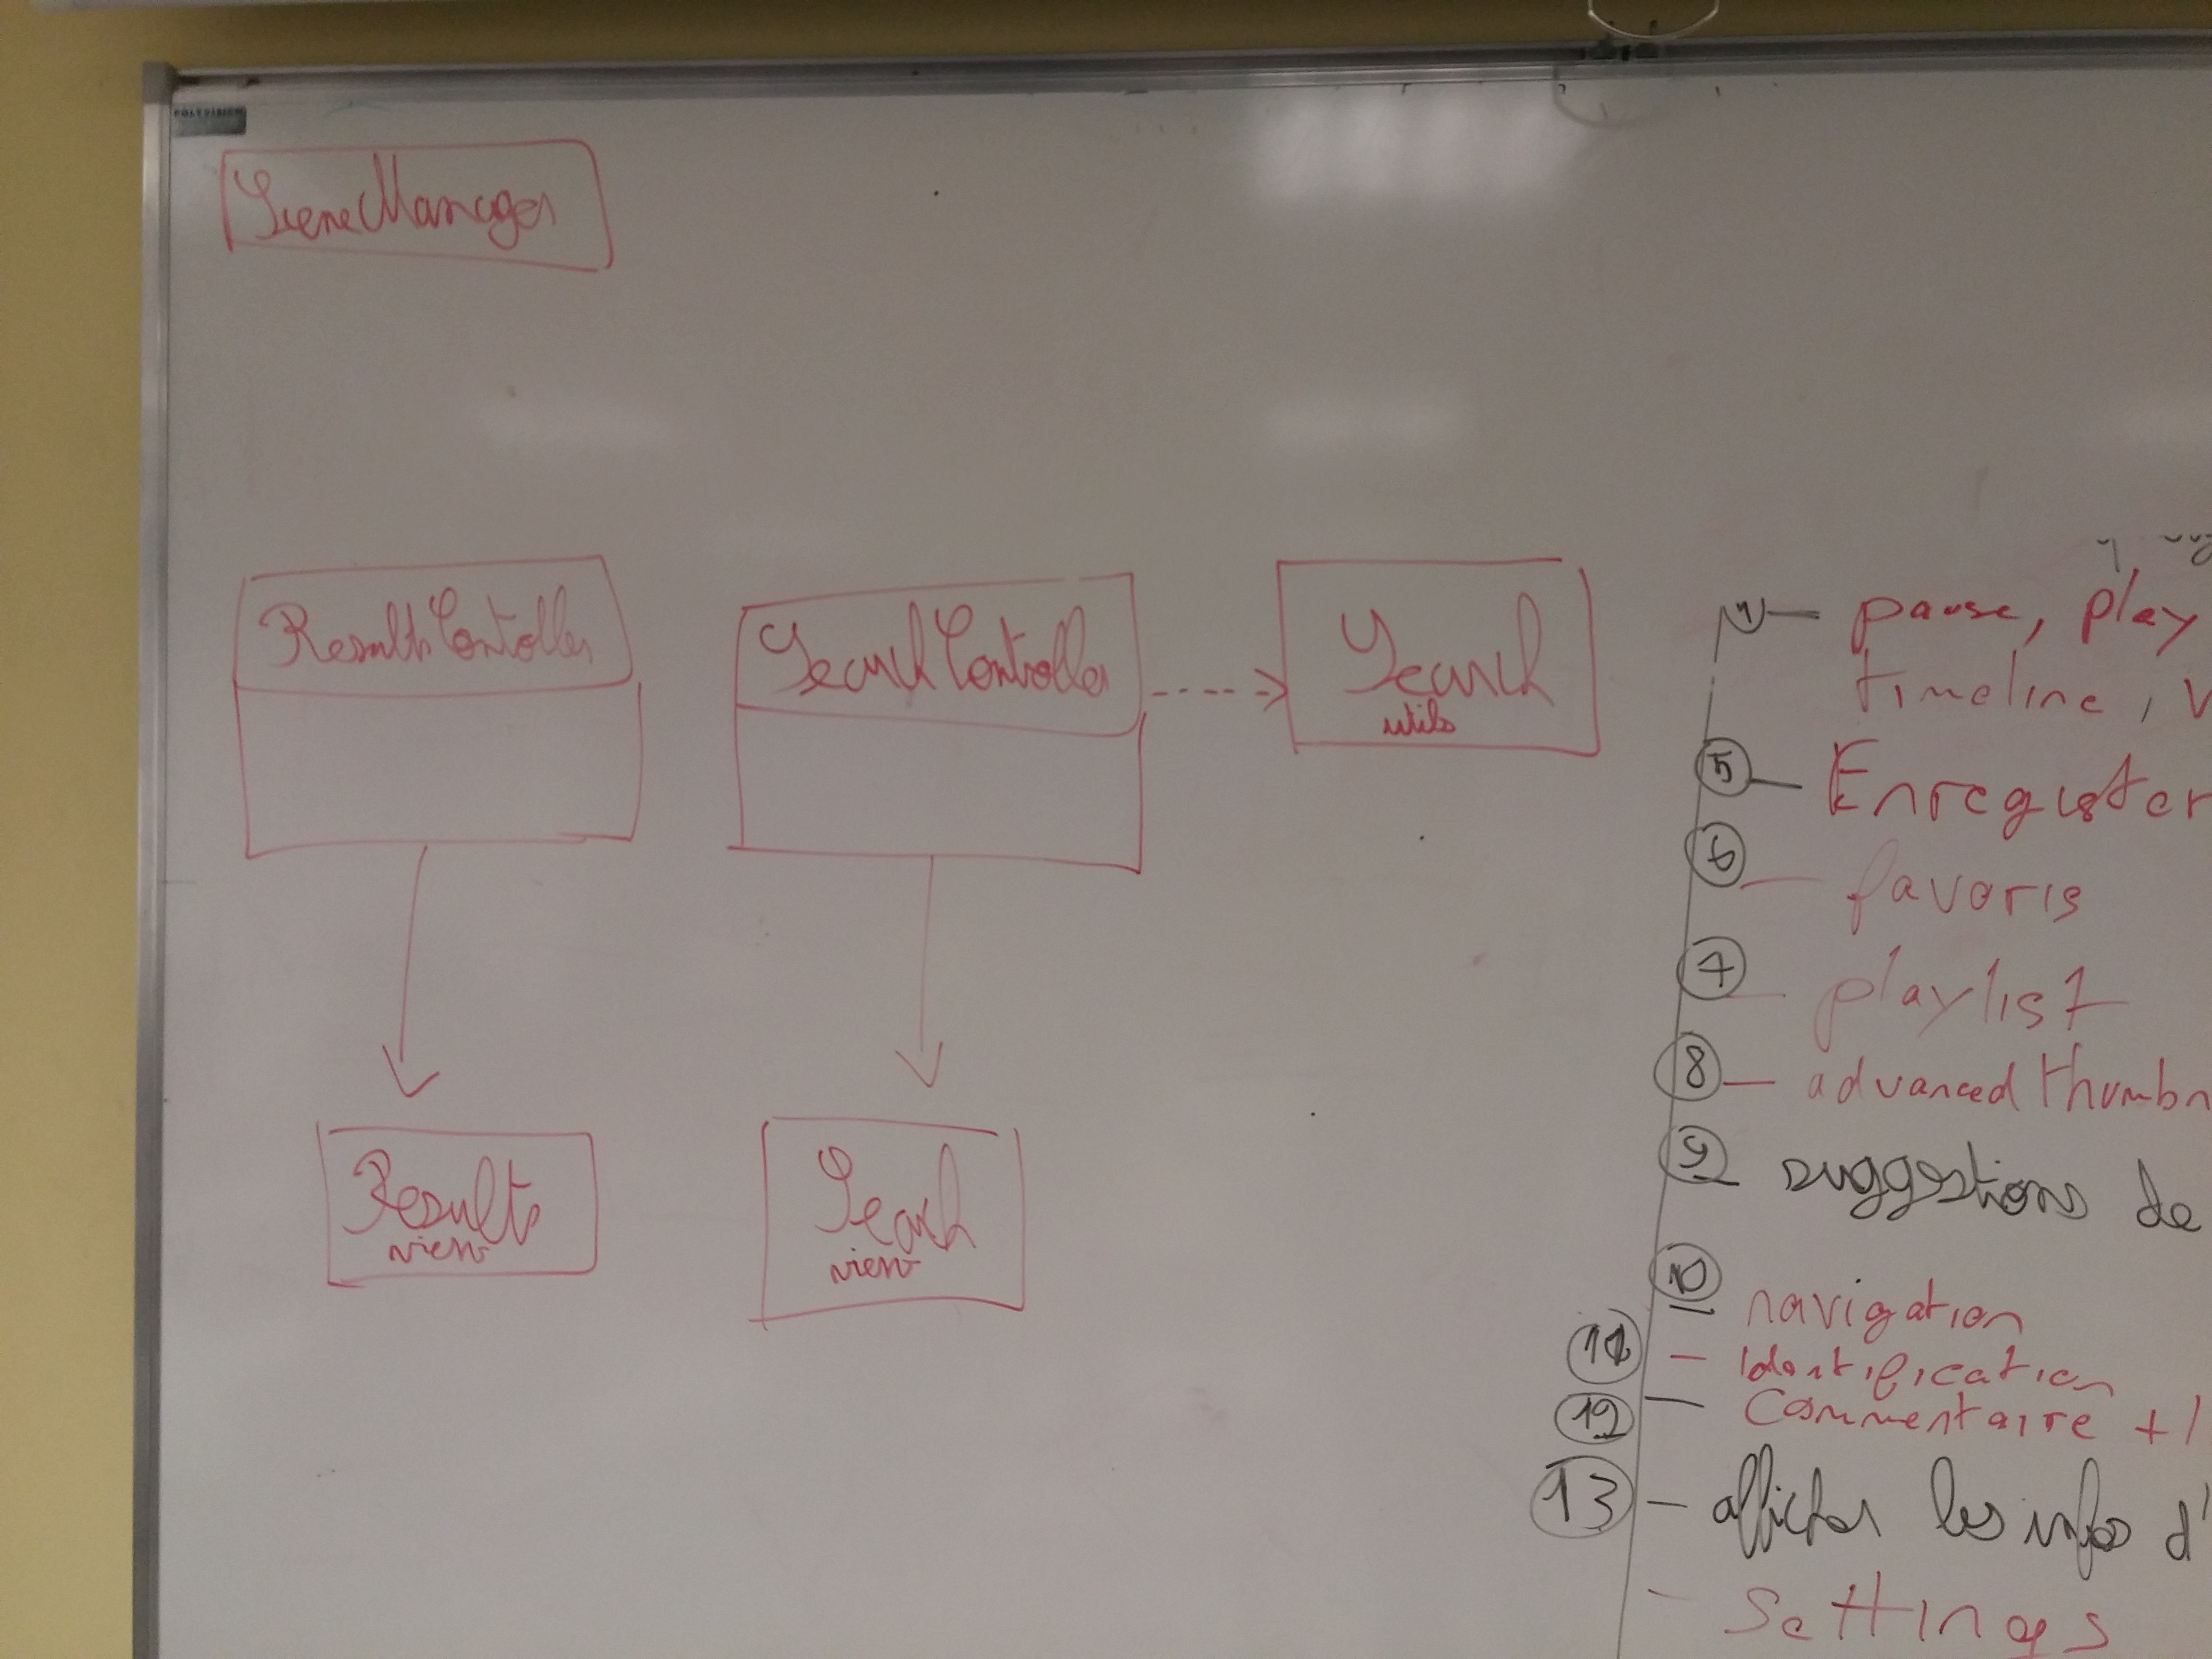
\includegraphics[width=0.8\textwidth]{1.jpg}
\end{center}

À la fin de cette journée, nous avons pu développer la fonctionnalité 1, 2 dans leur majorité. La fonctionnalité 4 est en cours de finition.


\begin{textblock}{0}(20, 190)
	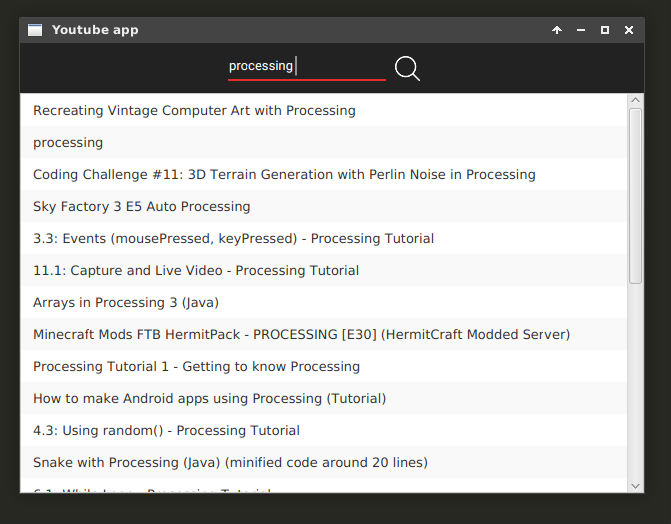
\includegraphics[width=\size, keepaspectratio]{V1.jpg}
\end{textblock}

\begin{textblock}{0}(105, 190)
	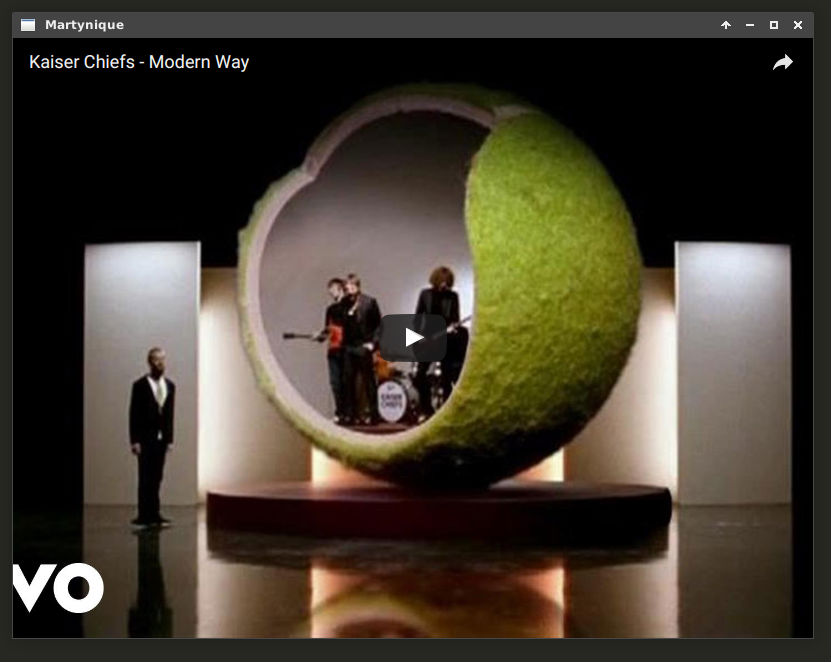
\includegraphics[width=\size]{V1_1.jpg}
\end{textblock}